\dots

\subsection{Utledning av Bølgelikningen} 
\subsubsection{Forhåndsbetingelser}
For å finne frem til bølgelikningen, må en se på hvordan systemet en skal bruke likningen i ser ut, 
På en gitar er lengden på strengen justerbar, men en endrer tonen ved å endre stramme eller slakke
ut på gitarstrengen. 

En gitarstreng kan modelleres som en tråd som er spennt mellom to punkter, der den er fiksert på plass. 
I normaltilstand ligger strengen spent i en rett linje mellom punktene, frem til den blir plukket. Da
har den blitt forstyrret, og strengen begynner å vibrere. Problemet er da å finne en $u(x,t)$ som modellerer
defleksjonen til strengen. Hvis strengen har lengde $l$ og blir sluppet løs ved $t=0$, vil formelen finne
defleksjonen til strengen for hvilken som helst $x$ når $t>0$. 

For å løse likningen trengs det noen forhåndsbetingelser.

\begin{enumerate}
	\item Gravitasjon er neglisjerbare i forhold til strengspenningen.
	\item Alle defleksjoner er små, og skjer i samme plan.
	\item Massen av strengen per lengde er konstant over hele strengen, slik at spenningen er den samme 
	gjennom hele strengen.
\end{enumerate}

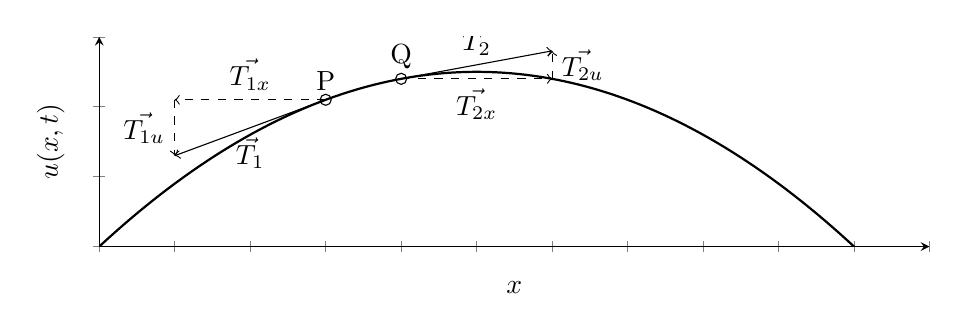
\begin{tikzpicture}
	\begin{axis} [
		width = \textwidth,
		height = 0.35\textwidth,
		axis lines = left,
		xlabel = \(x\),
		ylabel = {\(u(x, t)\)},
		xmin = 0, xmax = 1.1,
		ymin = 0, ymax = 0.6,
		xticklabel = \empty,
		yticklabel = \empty,
	]

	\addplot [
		domain = 0:1,
		samples = 100,
		color = black,
		thick,
	]
	{-2*x^2 + 2*x};

	\draw[->, thin, black] (axis cs:0.3,0.42) -- (axis cs:0.1,0.26) node[midway, below] {$\vec{T_1}$};
	\draw[->, thin, dashed, black] (axis cs:0.3,0.42) -- (axis cs:0.1,0.42) node[midway, above] {$\vec{T_{1 x}}$};
	\draw[->, thin, dashed, black] (axis cs:0.1,0.42) -- (axis cs:0.1,0.26) node[midway, left] {$\vec{T_{1 u}}$};

	
	\draw[->, thin, black] (axis cs:0.4,0.48) -- (axis cs:0.6,0.56) node[midway, above] {$\vec{T_2}$};
	\draw[->, thin, dashed, black] (axis cs:0.4,0.48) -- (axis cs:0.6,0.48) node[midway, below] {$\vec{T_{2 x}}$};
	\draw[->, thin, dashed, black] (axis cs:0.6,0.48) -- (axis cs:0.6,0.56) node[midway, right] {$\vec{T_{2 u}}$};

	\draw[dashed, black] (axis cs:0.3,0) -- (axis cs:0.3,0,42) node[below] {$x$};
	\draw[dashed, black] (axis cs:0.4,0) -- (axis cs:0.4,0,48) node[below] {$x + \Delta x$};

	\addplot [
		only marks,
		mark=o,
		color=black,
		nodes near coords,
		point meta=explicit symbolic,
	] coordinates {
		(0.3,0.42) [P] 
		(0.4,0.48) [Q]};
	
	\end{axis}
\end{tikzpicture}


% Forhåndsbetingelser:
% 1. Gravitasjon er neglisjerbart i forhold til strengspenningen
% 2. Alle defleksjoner er "små" altså vi kan bruke "jukseregler" på vinkler
% 3. Spenningen er lik på hele strengen

% Dette gjør at på et strengsegment er kansellerer de horisontale komponentene hverandre ut,
% og det kun er den vertikale akksellerasjonen vi må tenke på






\subsection{Valg av løsningmetode for numerisk løsning}
\subsubsection{Valg av verktøy}
\dots

\subsubsection{Implementasjon av bølgeligningen}
\dots





\subsection{Beskrivelse av kode for numerisk løsning}
\subsubsection{Programmets struktur og oppbygning}
\dots

\subsubsection{Hvordan programkoden og visualiseringen opererer}
\dots

